\documentclass{standalone}
\begin{document}
\markboth{CHAPTER 1. MATERIALS AND METHODS}{1.6. SVCs}
\section{Support Vector Classifiers}

Support Vector Classifiers (SVCs) are a subclass of Support Vector Machines (SVMs) that are a set of supervised learning methods (i.e. requires training data) used for purposes such as classification and regression.
A Support Vector Machine constructs a hyper-plane or set of hyper-planes in a high or infinite dimensional space.
Intuitively, a good separation is achieved by the hyper-plane that has the largest distance to the nearest training data points of any class (functional margin), since in general the larger the margin the lower the generalization error of the classifier\cite{SVCscikit, Bishop}.\\
For a SVC, mathematically, given training vectors $ \mathbf{x}_i \in \mathbb{R}^p ,  \: i \in \{1,\dots, n\} \:$, in two classes, and a vector $\mathbf{y} \in \{ -1, \: 1 \}^n$ (or $ \{0, \: 1 \}^n$), the goal is to find $\mathbf{w} \in \mathbb{R}^p$ and $b \in \mathbb{R}$ such that the prediction given by $sign(\mathbf{w^T  \mathbf{\Phi(x)}} + b)$ is correct for most samples \cite{SVCscikit}.\\
The function $\Phi(x)$ provides a convenient way of extending the analysis from the input space to a non-linear feature space by using a high-dimensional mapping. 
Finding a linear separating hyperplane in this feature space is equivalent to finding a non linear decision boundary in the input space\cite{SVCmapping}.\\
A SVC solves a primal problem and a dual problem. 
The primal:
\begin{equation}
    \min_{w, \zeta} \frac{1}{2} (\mathbf{w}^T  \mathbf{w}) + C \sum_{i = 1}^{n} \zeta_i
\end{equation}

subject to: $\begin{cases}
    y_i \cdot (\mathbf{w}^T  \mathbf{\Phi(x_i)} + b)  \geq 1 - \zeta_i, \\
    \zeta_i \geq 0 \quad i = 1, \dots, n 
    \end{cases}$
\newline
\\
\\
From an intuitive point of view, the minimization ($\mathbf{w}^T  \mathbf{w}$) corresponds to maximize the functional margin while incurring a penalty when a sample is misclassified or within the margin boundary.
The penalty term C controls the strength of this penalty, and acts as an inverse regularization parameter\cite{SVCscikit}.
Ideally, the term $\zeta_i$ should be 0 for a perfect prediction but real data are usually not always perfectly separable with a hyperplane, so some samples will be at a distance $\zeta_i$ from their correct margin boundary.
\\
The dual problem instead:
\begin{equation}
    \min_{\alpha} \frac{1}{2} (\mathbf{a}^T \mathbf{Q} \mathbf{a}) - \mathbf{e}^T \mathbf{a}
\end{equation}

subject to: $\begin{cases}
    \mathbf{y}^T \mathbf{a} = 0, &  \\
    0 \leq a_i \leq C  &  i = 1, \dots, n
    \end{cases}$
\newline
where $\mathbf{e}$ is the vector of all ones, $\mathbf{Q}$ is a $n \times n$ matrix: $Q_{ij}\equiv y_i y_j K(\mathbf{x_i}, \mathbf{x_j})$ where $K(\mathbf{x_i}, \mathbf{x_j}) = \mathbf{\Phi(x_i)}^T \mathbf{\Phi(x_j)} $ is the so called \textit{kernel}.
The $a_i$ terms are called \textit{dual coefficients}, and they are upper-bounded by C.\\


\newpage
\markboth{CHAPTER 1. MATERIALS AND METHODS}{1.6. SVCs}
Once these problems are solved, for a sample $\mathbf{z}$, the decision function is given by: 
\begin{equation}
    \sum_{i \in SV}^{}  y_i a_i \mathbf{K(x_i, z)} + b
\end{equation}
where the sum is over the supported  vectors (SV) that are the samples that lie within the margin because the dual coefficients $a_i$ are zero for the other samples\cite{SVCscikit}.

\begin{figure}[ht]

    \centering
    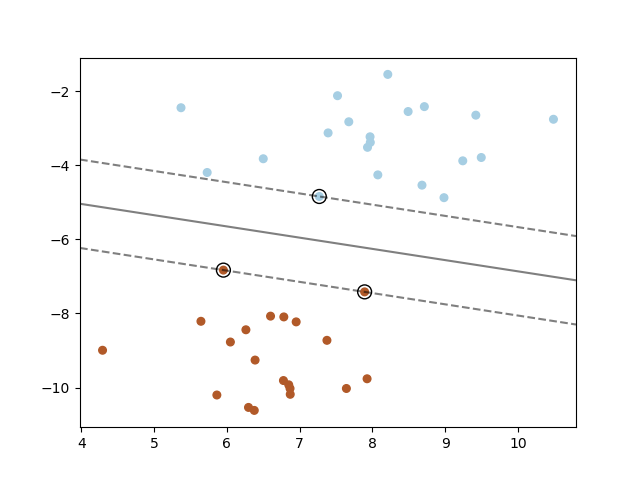
\includegraphics[width=.95\textwidth]{../images/svcexample.png}
    
    \caption{Classification made by a Support Vector Classifier (SVC) for a linearly separable problem. The gray line represents the line of the separation hyper-plane. The three samples on the margin boundaries (dashed lines) are called \textit{support vectors}. From \cite{SVCscikit}}\label{fig:svc}
    
    
    \end{figure}

\end{document}